\section{Workflow overview}


%{ % all template changes are local to this group.
    %\setbeamertemplate{navigation symbols}{}
    %\begin{frame}<article:0>[plain]
        %\vfill

        %\begin{center}
            %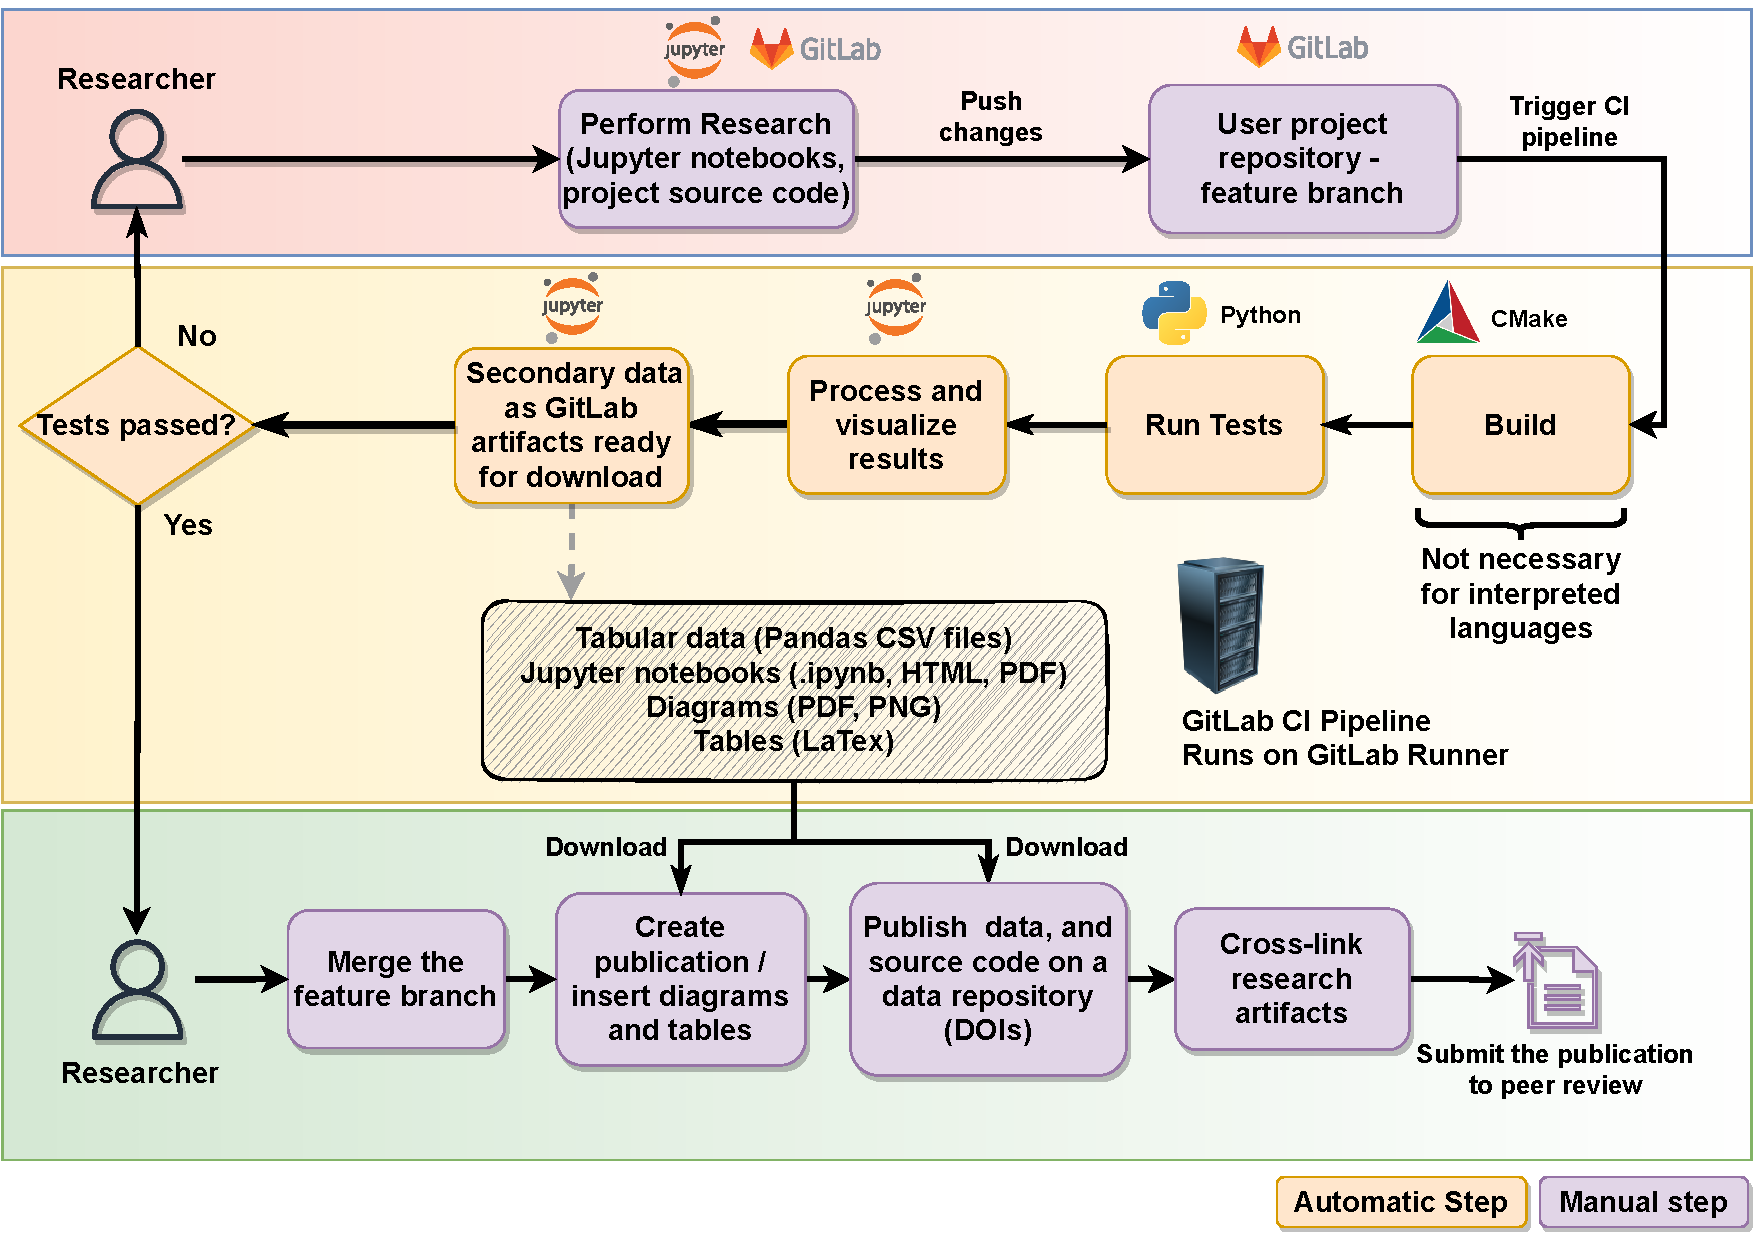
\includegraphics[width=0.75\textwidth]{figures/ZINF-CI-diagram-individual.drawio.pdf}
        %\end{center}
        %{\tiny \href{https://doi.org/10.6084/m9.figshare.16601282.v2}
        %{https://doi.org/10.6084/m9.figshare.16601282.v2}}
     %\end{frame}
%}

%{ % all template changes are local to this group.
    %\setbeamertemplate{navigation symbols}{}
    %\begin{frame}<article:0>[plain]
        %\vfill

        %\begin{center}
        %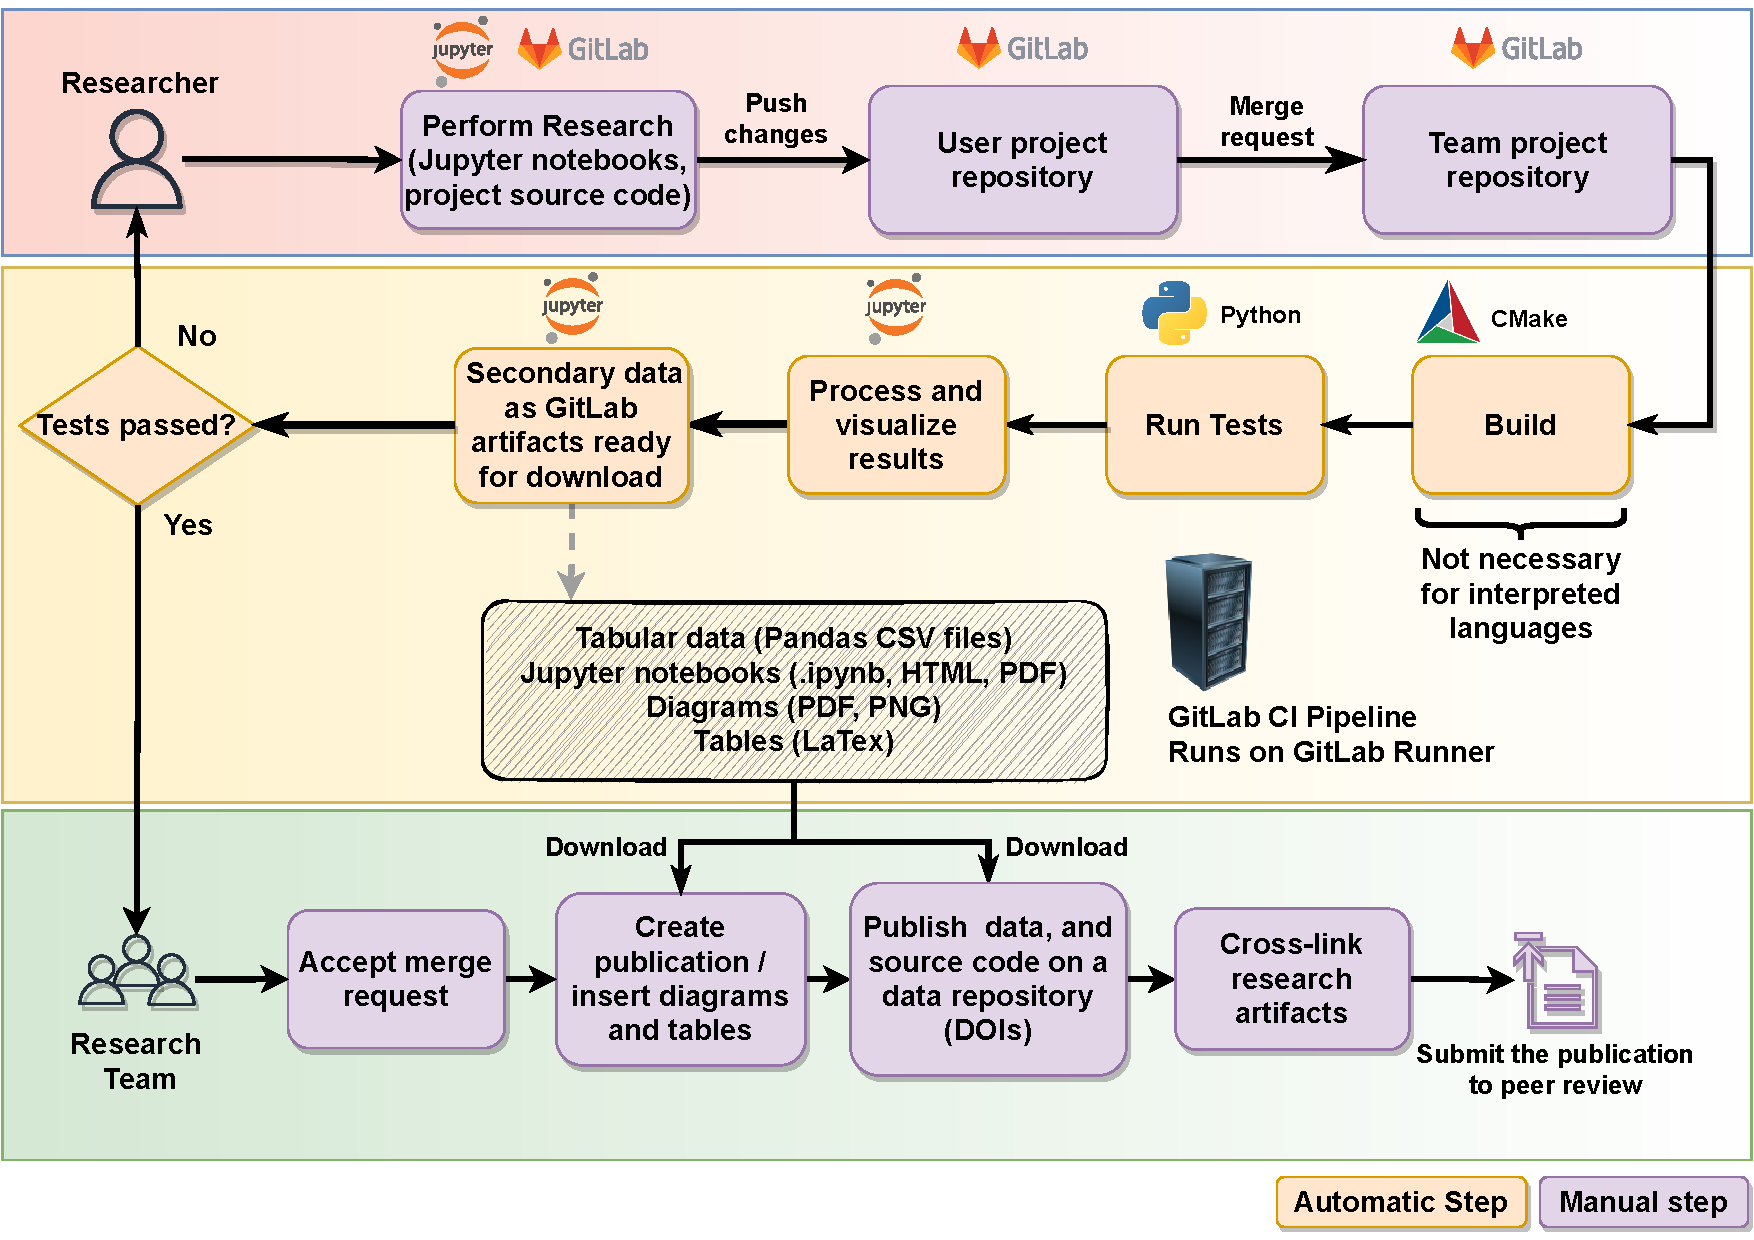
\includegraphics[width=0.75\textwidth]{figures/ZINF-CI-diagram.drawio.pdf}
        %\end{center}
        %{\tiny \href{https://doi.org/10.6084/m9.figshare.16601282.v2}
        %{https://doi.org/10.6084/m9.figshare.16601282.v2}}
     %\end{frame}
%}

%\begin{frame}{A workflow for increasing the quality of scientific CSE software} 


%\end{frame}

%\begin{frame}{A workflow for increasing the quality of scientific CSE software} 

    %\vfill
    %The workflow is using GitLab, specifically \href{https://git.rwth-aachen.de/}{TUGitLab}. 
    %Optional steps are in round () brackets.
    %\begin{enumerate}
        %\item Track the issues in a Kanban board. 
            %\begin{itemize}
                %\item Model issues as \href{https://betterscientificsoftware.github.io/PSIP-Tools/PTCs/}{Progress Tracking Cards}\footnote{Developed by \href{https://bssw.io/}{Better Scientific Software.}}.
            %\end{itemize}
        %\item Use version-control with a simple branching model. 
        %\item (Apply Test-Driven Development (TDD) for CSE software.)
        %\item (Enable Continuous Integration with an emphasis on result visualization.) 
        %\item Cross-link software, result data, and report/article when reaching a milestone.
            %\begin{itemize}
                %\item When submitting a publication to peer-review. 
                %\item After the publication has been accepted. 
                %\item When giving up on an idea. 
            %\end{itemize}
        %\item (Publish a Singularity image with the code and data.)
    %\end{enumerate}
%\end{frame}

%\begin{frame}{A workflow for increasing the quality of (academic) CSE software} 
    %\framesubtitle{OpenFOAM}

        %\vfill

        %The workflow is developed with OpenFOAM projects in mind, but it is tested with other research software. 

        %\vspace{1cm}

        %\textbf{Disclaimer}: This offering is not approved or endorsed by OpenCFD Limited, producer and distributor of the OpenFOAM software via www.openfoam.com, and owner of the OPENFOAM®  and OpenCFD®  trade marks. 

%\end{frame}
